\documentclass[12pt]{article}

\usepackage{amsmath}
\usepackage[hidelinks]{hyperref}
\usepackage{fancyhdr}
\usepackage{color}
\usepackage{titlesec}
\usepackage[pdftex]{graphicx}
\usepackage{datetime}

\pagestyle{fancy}
\fancyhf{}

% custom section
\titlespacing{\section}{0pt}{*2}{0pt}
\titleformat{\section}[runin]
{\normalfont\bfseries}
{\thesection. }
{0pt}
{}[\\]

\begin{document}

\fancyhead[L]
{
\textbf{Distributed Algorithms: Assignment 3 C}\\
Christos Froussios (4322754) \& Quinten Stokkink (4016270)\\
\today
}
\setlength\headheight{0.8in}
\setlength\topmargin{-0.6in}
\setlength\textheight{9.0in}
\setlength\parindent{0pt}

\section{Introduction}
In this report we present the results of our implemenation of Afek \& Gafni's algorithm for election in a completely connected network.
We use a slightly modified version of the algorithm to avoid drowning single processes in so many messages they slow down the
whole algorithm. This involves selecting from the untraversed link pool in a random order and a timeout between trying to capture
the same node successively. Furthermore we demote candidate processes that have been killed and have no outstanding messages
to just an ordinary process.

\section{Methodology}
To test our algorithm we simulated a fully distributed environment by giving each process its own JVM environment.
This is quite costly for the simulating machine, but also far more accurate than testing between two or more
physical machines as every process has access to the exact same capabilities (and delays).
In fact through our tests we found that as the memory footprint nears 4 GB and the amount of threads gets close
to 10,000 our simulating machine starts locking up.

\quad As for our testing methodology we decided to always test the worst case, which occurs when all processes present themselves
as candidate processes and start the algorithm. By testing the worst cases we should see a curve of the runtime
that is in the order of $O(n log(n))$ as advertised by the algorithm.

\section{Results}
We have run tests for the amounts of processes (which are both candidates and ordinary processes at the same time) of:
1, 10, 20, 30, 50, 80, 100, 130 and 150. For each of these processes we then reported the level it reached and whether
it was elected (to verify correctness). For each of these experiments we also recorded the total time.

\quad The results of the running time experiments are visualized in \autoref{fig:totaltime} and the measurements of the
maximum levels are visualized in \autoref{fig:maxlevel}. We see that the running time does seem to follow an $O(n log(n))$ curve
and that the maximum levels reached seem to follow a linear curve.
Furthermore, \autoref{fig:captures} visualizes the total amount of captures performed in the algorithm versus the amount of
processes. While this series seems to follow a linear curve it suffers from a lot more noise than the other two metrics.

\quad Note that due to our optimization, candidates are only killed once. Therefore it does not make much sense to report on this.

\begin{figure}[p]
    \centering
    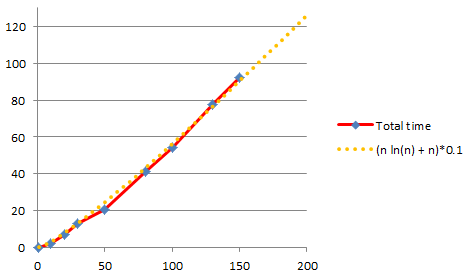
\includegraphics{totaltime.png}
    \caption{The total time taken for the algorithm to terminate versus the amount of processes}
    \label{fig:totaltime}
\end{figure}

\begin{figure}[p]
    \centering
    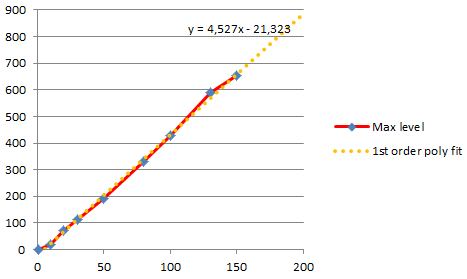
\includegraphics{maxlevel.png}
    \caption{The maximum level achieved versus the amount of processes}
    \label{fig:maxlevel}
\end{figure}

\begin{figure}[p]
    \centering
    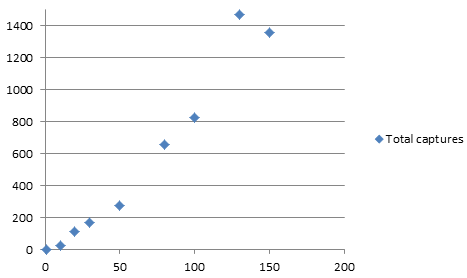
\includegraphics{totalcapture.png}
    \caption{The total amount of captures in the algorithm versus the amount of processes}
    \label{fig:captures}
\end{figure}

\end{document}